\documentclass[11pt]{article}
\usepackage[a4paper, margin=1in]{geometry}
\usepackage{graphicx}
\usepackage{tabularx}
\usepackage{amsmath}
\usepackage{hyperref}
\usepackage{fontawesome}

\title{Vision assignment 1}
\author{sumanasekarawkgg.19 }

\begin{document}

\thispagestyle{empty}
\begin{center}
   \begin{figure}
   \vspace*{1.5cm}
       \centering
       
\includegraphics[width=4.8cm]{Images/uom.png}
   \end{figure}
   
   Department of Electronic and Telecommunication Engineering \\ University of Moratuwa \\
   \vspace{2cm}
   {\fontsize{14}{17}\selectfont\textbf{\\Assignment I\\}}
    \vspace{8cm}
    190610E - Sumanasekara W.K.G.G. 
   \vspace{3cm}
   \\This report is submitted as a partial fulfillment of module EN2550
   \vspace{0.5cm} \\
   \today
\end{center}

\newpage
\clearpage
\pagenumbering{arabic} 

\noindent \textbf{Note}: All codes can be found in \faGithub{ \url{https://github.com/GevinduGanganath/EN2550/tree/main/Assignment%201}}

\section*{Question 1}

In the given intensity transformation, pixel values lie within the range 50 to 150 has been increased while other pixels remain same. 
Above pixel values of a gray scale image generally represent gray colour, hence we can observe that gray colour pixels have been 
transformed into near white in the output image. Figure \ref{Question 1} shows the original image, intensity transformation function and output image 
respectively.

\begin{figure}[!h]
    \centering
    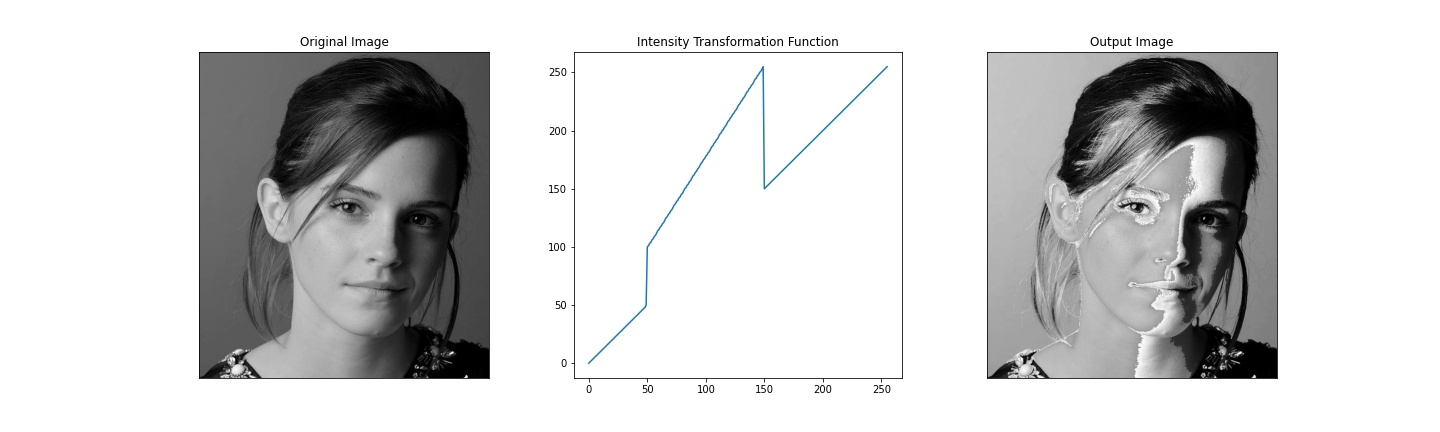
\includegraphics[width=\textwidth]{Images/1.jpg}
    \caption{Question 1}
    \label{Question 1}
\end{figure}

\section*{Question 2}

\begin{itemize}
    \item[(a)] In this part the white matter of brain proton density image has been accentuated. Applied intensity transformation is
               shown in figure \ref{Question 2-a}. Since both the white matter and gray matter \cite{brain} have closer pixel values it is very important 
               to select the correct cut-off value. Here 175 was selected as cut-off value and range between 150 and 200 has transformed 
               linearly while others are shifted to pure white or black.

                \begin{figure}[!h]
                    \centering
                    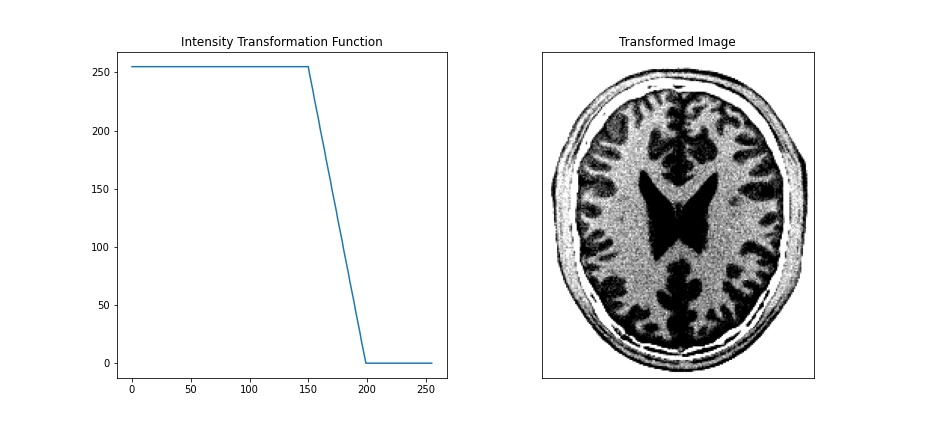
\includegraphics[width=\textwidth]{Images/2a.jpg}
                    \caption{Question 2-a}
                    \label{Question 2-a}
                \end{figure} 
    
    \item[(b)]  As the second part, gray matter of the image has been accentuated. Here the transformation is different from the previous one because
                if a transformation of the same shape is applied white matter also accentuated and then it is difficult to figure out the features of 
                gray matter. Corresponding transformation function and accentuated image is shown in figure \ref{Question 2-b}.

                \begin{figure}[!h]
                    \centering
                    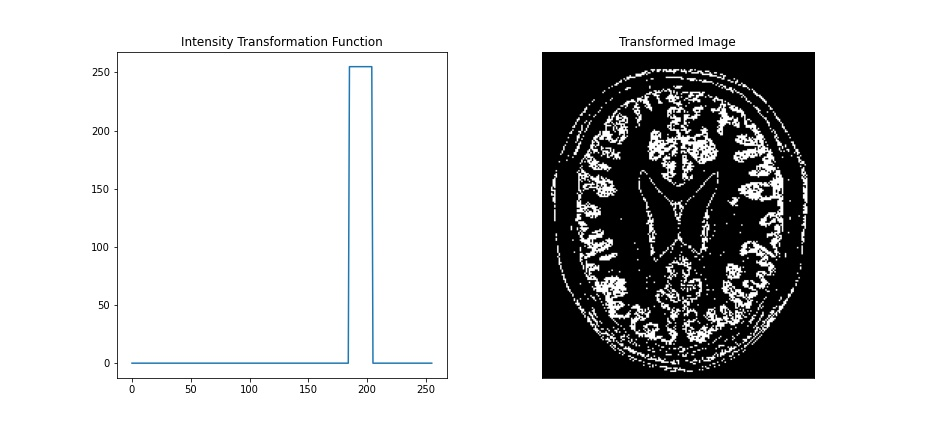
\includegraphics[width=\textwidth]{Images/2b.jpg}
                    \caption{Question 2-b}
                    \label{Question 2-b}
                \end{figure} 
\end{itemize}

\section*{Question 3}

In this exercise a gamma correction ($\gamma = 0.8$) has been performed on the L place of the given image after converting it to the L*a*b 
colour space \cite{lab}. Results are shown in figure \ref{Question 3 input and output images}.

\begin{figure}[!h]
    \centering
    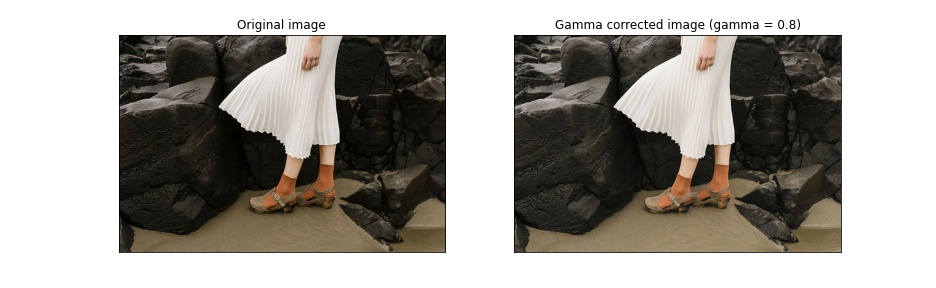
\includegraphics[width=\textwidth]{Images/31.jpg}
    \caption{Question 3 input and gamma corrected images}
    \label{Question 3 input and output images}
\end{figure}

\noindent In the L*a*b colour space L represents the lightness of the pixel. According to the equation \ref{eq:1} applying a gamma value less than
1 always produces a new L value which is grater than the previous. Therefore, after the gamma correction output image is lighter than before
giving a nice appearance to dark places like rock hallows. 

\begin{equation}\label{eq:1}
    \text{new L value} = 255\left(\frac{\text{current L value}}{255}\right)^{0.8}
\end{equation}

\noindent This can also be represented using the histograms of the two versions of image. As you can observe in figure \ref{Question 3 histograms},
after the gamma correction histogram has moved right slightly while storing more pixels in right most bins.

\begin{figure}[!h]
    \centering
    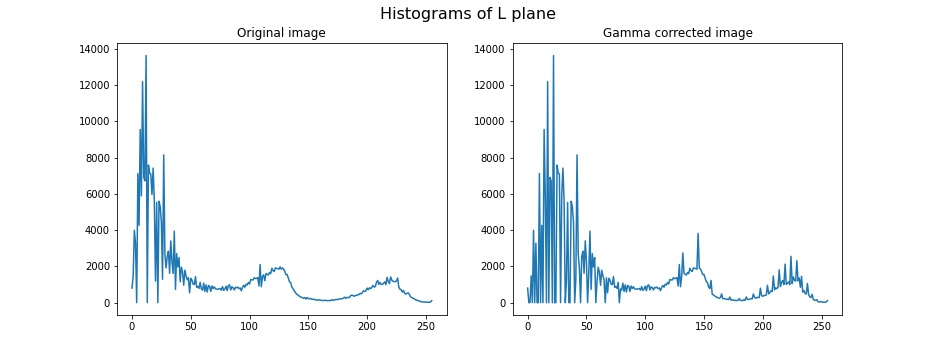
\includegraphics[width=\textwidth]{Images/32.jpg}
    \caption{Question 3 histograms}
    \label{Question 3 histograms}
\end{figure}

%\newpage
\section*{Question 4}

Images may have histograms confined into some region, but a histogram of a good image have the values in all regions. Therefore, we need to 
distribute the pixel values throughout the region. That is what histogram equalization does  \cite{histo}. \\

\noindent In this exercise a python function was written (figure \ref{Histogram Equalization Function}) to carry out the histogram equalization on a given image. As the first step histogram of the given image was
obtained using the numpy histogram function and the cumulative summation was calculated. Then the histogram equalization equation can be 
applied resulting a transformation function. Finally, it can be used as a look-up table to generate the equalized image.
Resulting histograms are shown in figure \ref{Histograms} and the proper operation of the implemented function can be verified by comparing it 
with the output of openCV in-built histogram equalization function. Equalized image is shown in figure \ref{41}.

\begin{figure}[!h]
    \centering
    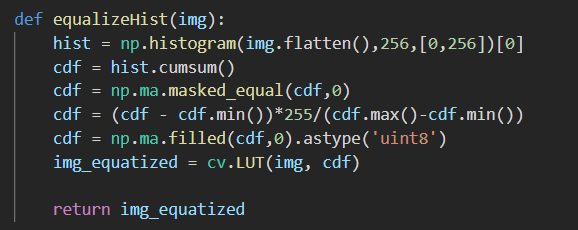
\includegraphics[width=0.7\textwidth]{Images/40.PNG}
    \caption{Histogram Equalization Function}
    \label{Histogram Equalization Function}
\end{figure}

\begin{figure}[!h]
    \centering
    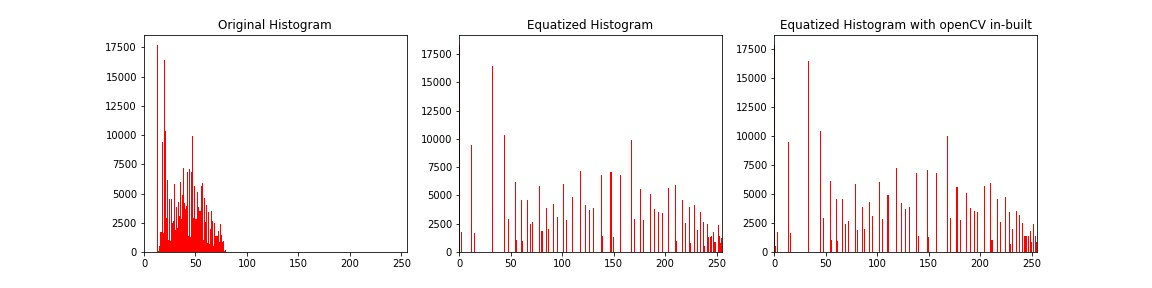
\includegraphics[width=\textwidth]{Images/42.jpg}
    \caption{Histograms of shell image}
    \label{Histograms}
\end{figure}

\begin{figure}[!h]
    \centering
    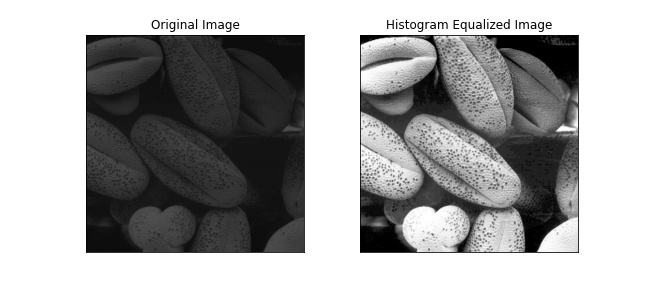
\includegraphics[width=\textwidth]{Images/41.jpg}
    \caption{Equalized image}
    \label{41}
\end{figure}

\section*{Question 5}

Two functions were implemented to carry out the zooming and calculate the normalized sum of squared difference (SSD). The zooming function is 
capable of handling the both nearest-neighbor and bilinear interpolation techniques. By observing the SSD values in table 1, we can conclude that 
bilinear interpolation provides the better results.

\begin{center}
    Table 1: SSD value comparison
    \begin{tabular}{ |c|c|c| } 
        \hline
        Image & SSD with nearest-neighbor interpolation & bilinear interpolation \\ 
        \hline
        Image 1 & 641.788 & 628.113 \\
        \hline
        Image 2 & 268.688 & 259.388 \\
        \hline
        Image 3 & 426.194 & 404.029 \\
        \hline
    \end{tabular}
\end{center}

\section*{Question 6}

\begin{itemize}
    \item[(a)] Here openCV filter2D function was used to carry out the sobel filter on Einstein image. Sobel kernels detect the
            edges of a given image. As can be observed in the figure \ref{51} Sobel vertical kernel detects the horizontal edges while 
            Sobel horizontal kernel detects the vertical edges. 
    
    \begin{figure}[!h]
        \centering
        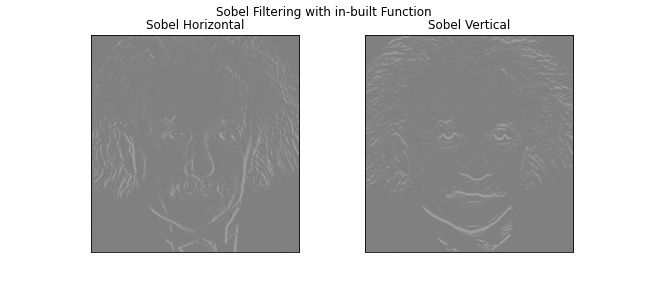
\includegraphics[width=\textwidth]{Images/51.jpg}
        \caption{Question 6-a}
        \label{51}
    \end{figure}
    
\end{itemize}

\section*{Question 7}

\begin{itemize}
    \item[(a)] Here a grabCut segmentation \cite{grabcut} was carried out to extract the background from the given image. Initially, I tried 
    the segmentation with bounding boxes, but it did not produce the expected output, specially closer to the flower bud and to the petals of flower 
    in question. Then a mask was generated by doing few modifications to the binary thresholded image and grabCut was carried out with mask approximation. 
    In this case the outputs were better than the previous. Results are shown in figure \ref{71}. 
                
    \begin{figure}[!h]
        \centering
        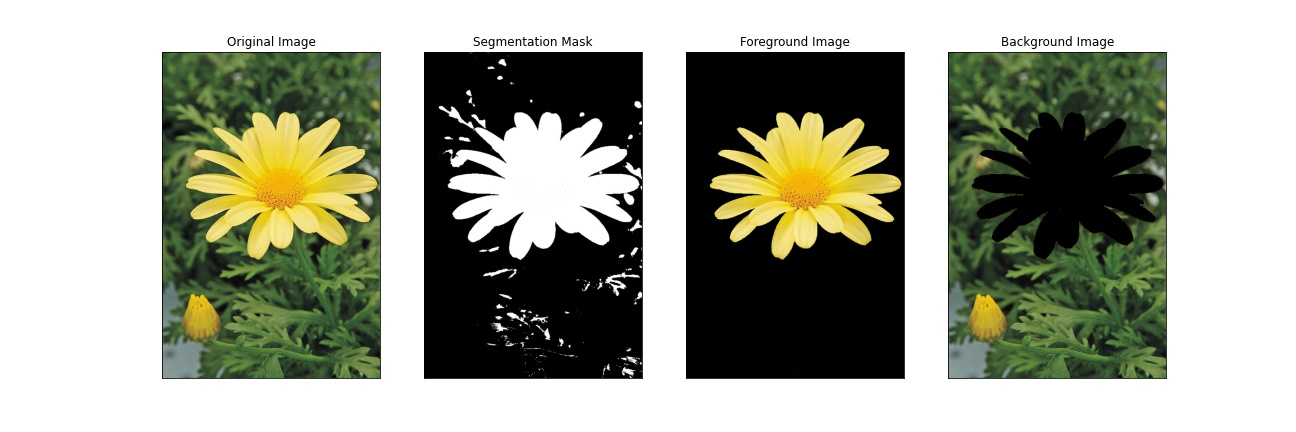
\includegraphics[width=\textwidth]{Images/71.jpg}
        \caption{Question 7-a}
        \label{71}
    \end{figure}

    \item[(b)] In the second part an enhanced image was produced by summing up the foreground image (saturation increased) and background image 
    (Gaussian blurred). Output is shown in figure \ref{72}. 
    
    \begin{figure}[!h]
        \centering
        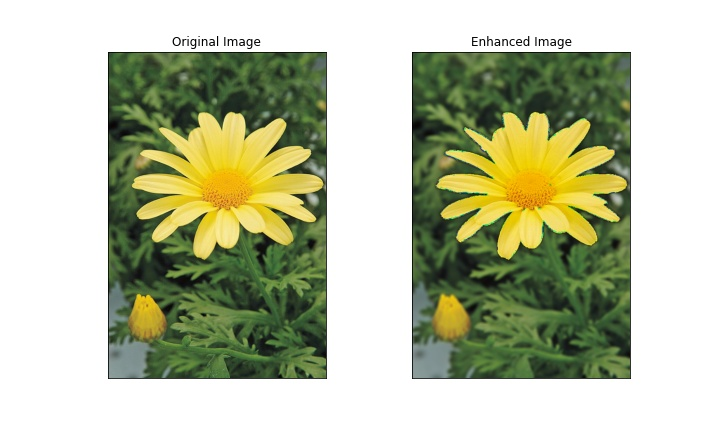
\includegraphics[width=\textwidth]{Images/72.jpg}
        \caption{Question 7-b}
        \label{72}
    \end{figure}
        
\end{itemize} 
    
\newpage
\bibliographystyle{IEEEtran}
\bibliography{ref}

\end{document}